\documentclass[tikz,border=10pt]{standalone}
\usepackage{tikz}
\usetikzlibrary{arrows.meta,positioning}

\begin{document}
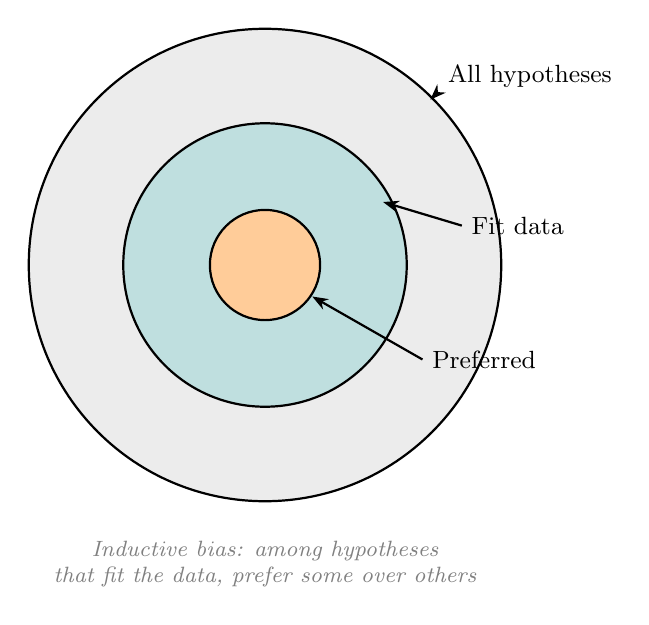
\begin{tikzpicture}[
    arrow/.style={-{Stealth[length=2mm]}, thick},
    label/.style={font=\small, align=left}
]

% Outer circle - All hypotheses
\fill[gray!15] (0,0) circle (3cm);
\draw[thick] (0,0) circle (3cm);

% Middle circle - Fit data
\fill[teal!25] (0,0) circle (1.8cm);
\draw[thick] (0,0) circle (1.8cm);

% Inner circle - Preferred
\fill[orange!40] (0,0) circle (0.7cm);
\draw[thick] (0,0) circle (0.7cm);

% Labels with arrows
\draw[arrow] (2.2, 2.2) -- (2.1, 2.1);
\node[label, right] at (2.2, 2.4) {All hypotheses};

\draw[arrow] (2.5, 0.5) -- (1.5, 0.8);
\node[label, right] at (2.5, 0.5) {Fit data};

\draw[arrow] (2.0, -1.2) -- (0.6, -0.4);
\node[label, right] at (2.0, -1.2) {Preferred};

% Caption-style label at bottom
\node[font=\footnotesize\itshape, text=gray, align=center] at (0, -3.8) {Inductive bias: among hypotheses\\that fit the data, prefer some over others};

\end{tikzpicture}
\end{document}
